\section{A worked eight-point example in 4D}
\label{app:eight}

This example explains the numerical objects before using them. A
\emph{cell} is a small rectangular region on which box membership is
constant. Its \emph{mass} is its ordinary volume. A \emph{mask} is a
zero-or-one rule that excludes a covered region. A \emph{contraction}
means summing out a coordinate. \emph{Compression} means grouping
consecutive coordinate cells and retaining their total masses, together
with any dependence between coordinates.

\subsection{Input, reference point, and the two projections}
Use the origin as anchor and interpret the following points as upper
corners: larger coordinates are better. Equivalently, for minimization
with reference $r=(6,6,6,6)$, use objective vectors $p^j=r-a^j$.
All coordinates of both sets lie in $\{1,2,3,4,5\}$.
\begin{center}
\begin{tabular}{@{}c@{\qquad}rrrr@{\qquad}c@{}}
\toprule
Point & $a_1$ & $a_2$ & $a_3$ & $a_4$ & Coordinate sum\\\midrule
$a^1$ &5&1&5&1&12\\
$a^2$ &5&2&3&2&12\\
$a^3$ &4&3&4&1&12\\
$a^4$ &3&4&2&3&12\\
$a^5$ &2&5&1&4&12\\
$a^6$ &1&5&2&4&12\\
$a^7$ &2&2&5&3&12\\
$a^8$ &1&3&3&5&12\\\bottomrule
\end{tabular}
\end{center}
No point dominates another: distinct vectors with the same coordinate
sum cannot be coordinatewise larger than one another. Their boxes
nevertheless overlap. The enclosing box is $[0,5]^4$, of volume $625$.

\begin{figure}[h!]
\centering
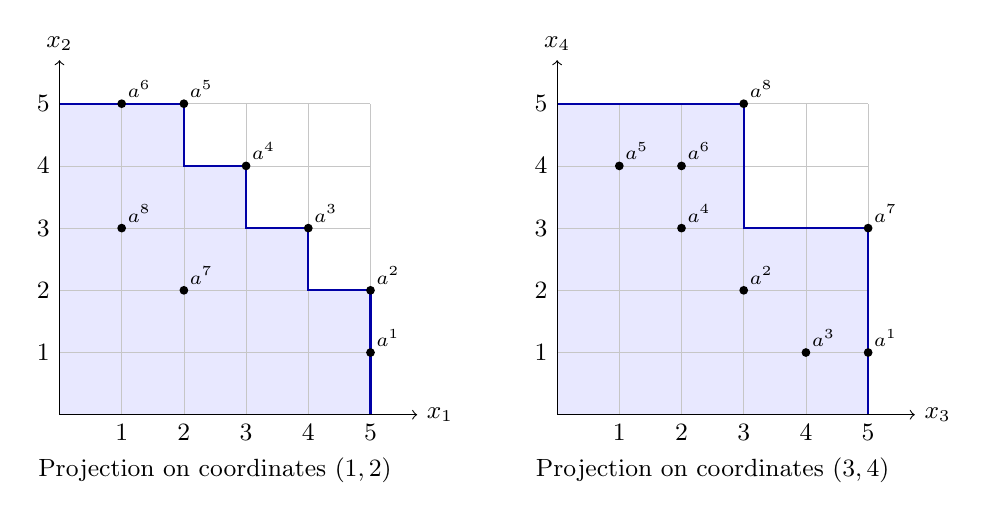
\begin{tikzpicture}[scale=.79, every node/.style={font=\small}]
\begin{scope}
\fill[blue!9] (0,0)--(5,0)--(5,2)--(4,2)--(4,3)--(3,3)--(3,4)--(2,4)--(2,5)--(0,5)--cycle;
\draw[step=1,gray!45,very thin] (0,0) grid (5,5);
\draw[blue!65!black,thick] (5,0)--(5,2)--(4,2)--(4,3)--(3,3)--(3,4)--(2,4)--(2,5)--(0,5);
\draw[->] (0,0)--(5.75,0) node[right] {$x_1$};
\draw[->] (0,0)--(0,5.7) node[above] {$x_2$};
\foreach \k in {1,...,5} {\node[below] at (\k,0) {\k};\node[left] at (0,\k) {\k};}
\foreach \x/\y/\lab in {5/1/1,5/2/2,4/3/3,3/4/4,2/5/5,1/5/6,2/2/7,1/3/8}
{\fill (\x,\y) circle (2pt);\node[above right,inner sep=2pt] at (\x,\y) {\scriptsize $a^{\lab}$};}
\node at (2.5,-.9) {Projection on coordinates $(1,2)$};
\end{scope}
\begin{scope}[xshift=8cm]
\fill[blue!9] (0,0)--(5,0)--(5,3)--(3,3)--(3,5)--(0,5)--cycle;
\draw[step=1,gray!45,very thin] (0,0) grid (5,5);
\draw[blue!65!black,thick] (5,0)--(5,3)--(3,3)--(3,5)--(0,5);
\draw[->] (0,0)--(5.75,0) node[right] {$x_3$};
\draw[->] (0,0)--(0,5.7) node[above] {$x_4$};
\foreach \k in {1,...,5} {\node[below] at (\k,0) {\k};\node[left] at (0,\k) {\k};}
\foreach \x/\y/\lab in {5/1/1,3/2/2,4/1/3,2/3/4,1/4/5,2/4/6,5/3/7,3/5/8}
{\fill (\x,\y) circle (2pt);\node[above right,inner sep=2pt] at (\x,\y) {\scriptsize $a^{\lab}$};}
\node at (2.5,-.9) {Projection on coordinates $(3,4)$};
\end{scope}
\end{tikzpicture}
\caption{Each label refers to the same 4D point in both plots. Shading
shows the union of projected anchored rectangles. Its areas are $19$
and $21$, respectively. Their product, $399$, is not the 4D hypervolume.}
\label{fig:eight-projections}
\end{figure}
\clearpage
\subsection{A hand-checkable calculation using the $2+2$ grouping}
The projections discard which pair belongs with which other pair.
For example, cell $(5,2)$ belongs to the left projection and cell $(3,5)$
to the right, but no input point covers the 4D cell $(5,2,3,5)$.

Every axis has coordinates $0,1,2,3,4,5$. For positive rank $k$ the cell
is $(k-1,k]$ and its length is $1$. The endpoint cell $\{0\}$ has
length zero and may be omitted in this ordinary-HV calculation.
Thus a positive-rank 4D cell has volume $1$.

Fix ranks $(i,j)$ in coordinates $(1,2)$. Only points with
$a_1\ge i$ and $a_2\ge j$ cover that first pair of cells. Let
\[
 H(i,j)=\HV_2\bigl(\{(a_3,a_4):a\in A,\ a_1\ge i,\ a_2\ge j\}\bigr).
\]
This is the area covered in the other two coordinates, conditional on
the chosen first pair. The word ``conditional'' here means selecting
the eligible points; it does not refer to a probability distribution.
All first-pair cells have area $1$, so
\[
                    \HV_4(A)=\sum_{i=1}^5\sum_{j=1}^5 H(i,j).
\]
The table can be checked by drawing the eligible rectangles in the
right-hand plot of Figure~\ref{fig:eight-projections}:
\begin{center}
\begin{tabular}{@{}c|rrrrr|r@{}}
\toprule
 & $j=1$&$j=2$&$j=3$&$j=4$&$j=5$&Row sum\\\midrule
$i=1$&21&21&16&8&8&74\\
$i=2$&16&16&9&7&4&52\\
$i=3$&10&9&8&6&0&33\\
$i=4$&8&7&4&0&0&19\\
$i=5$&8&6&0&0&0&14\\\bottomrule
\end{tabular}
\end{center}
For example, at $(i,j)=(2,3)$ the eligible points are $a^3,a^4,a^5$.
Their last two coordinates are $(4,1),(2,3),(1,4)$.
In the $x_3$ direction, the covered heights in $x_4$ are $4,3,1,1,0$.
Therefore $H(2,3)=4+3+1+1=9$. At $(5,2)$ only $a^2$ remains, and
$H(5,2)=3\cdot2=6$. Summing the rows gives
\[
               \boxed{\HV_4(A)=74+52+33+19+14=192.}
\]

\paragraph{What replaces integration?}
Let $W(t)=\sum_{s=1}^t1=t$, with $W(0)=0$. This is a prefix sum:
one stored cumulative mass for every endpoint. An interval of ranks
$q,\ldots,h$ has mass $W(h)-W(q-1)$ when $q\le h$, and zero otherwise.
It is exactly the integral of the unit density over those cells.
For instance, ranks $2,3$ have mass $W(3)-W(1)=3-1=2$.
No approximation of a continuous integral is involved.

The table above is an independent explanation and check, not the
data structure used by the fast algorithm. Constructing every such
table for a large input would not establish Chan's bound. The numerical
solver instead stores separate arrays and constraints and sums them
within the geometric recursion, as shown next.

\clearpage
\subsection{The actual recursion and its first absorbed box}
The solver computes the \emph{uncovered} volume $U$ inside $[0,5]^4$
and returns $625-U$. A simple box can be absorbed into a mask: the
box is removed from the list, while the mask remembers precisely which
cells must be excluded from subsequent sums.

At the root, $a^1=(5,1,5,1)$ reaches the enclosing boundary on axes
1 and 3. Only coordinates 2 and 4 restrict its coverage. On positive
ranks, its complement is
\[
 F(k)=\ind[k_2>1\ \text{or}\ k_4>1]
     =\ind[k_4\ge q(k_2)],\qquad
 q(j)=\begin{cases}2,&j=1,\\1,&j=2,3,4,5.\end{cases}
\]
The remaining seven boxes are initially hard: each still restricts at
least three coordinates. The prefix-sum calculation must keep $F$;
otherwise cells covered by $a^1$ would be counted as uncovered.

With the default base size of two hard boxes, the local compiled solver
chooses the following cuts. $L$ and $R$ mean the lower and upper child
of a cut. The table gives original positive ranks, rather than the
shifted local indices used internally after cropping arrays. A star
means the full positive range $1{:}5$.
\begin{center}
\small
\begin{tabular}{@{}lccccrl@{}}
\toprule
Node&$k_1$&$k_2$&$k_3$&$k_4$&$U$&Next operation\\\midrule
Root&$*$&$*$&$*$&$*$&433&Cut axis 1 after 3\\
$L$&$1{:}3$&$*$&$*$&$*$&216&Cut axis 2 after 3\\
$LL$&$1{:}3$&$1{:}3$&$*$&$*$&99&Cut axis 3 after 2\\
$LLL$&$1{:}3$&$1{:}3$&$1{:}2$&$*$&21&Base, two hard boxes\\
$LLR$&$1{:}3$&$1{:}3$&$3{:}5$&$*$&78&Base, two hard boxes\\
$LR$&$1{:}3$&$4{:}5$&$*$&$*$&117&Cut axis 3 after 2\\
$LRL$&$1{:}3$&$4{:}5$&$1{:}2$&$*$&27&Base, one hard box\\
$LRR$&$1{:}3$&$4{:}5$&$3{:}5$&$*$&90&Base, no hard boxes\\
$R$&$4{:}5$&$*$&$*$&$*$&217&Base, two hard boxes\\\bottomrule
\end{tabular}
\end{center}
These are the weighted-median cuts of Section~\ref{sec:geometry},
recorded from the implementation, not a separately chosen sweep.
For example, $99=21+78$, $117=27+90$, and $216=99+117$.
At the root, $U=216+217=433$, giving $625-433=192$.

There are four cuts, nine visited nodes, and five base evaluations.
After a cut, more boxes may become simple because they reach a new
cell boundary. Their masks remain in the numerical state even after
their generators leave the hard-box list. The table's $U$ is the
original uncovered volume in that region, including all inherited masks.
This small instance finishes before any scheduled compression occurs.
We illustrate compression separately below rather than claiming that
this run exercises it.

\clearpage
\subsection{One complete leaf calculation using numerical arrays}
Consider node $R$, where $k_1\in\{4,5\}$. Points $a^4,\ldots,a^8$
are disjoint from this region because their first coordinate is at most
3. Box $a^1$ has already become the mask $F$. Only $a^2$ and $a^3$
remain as hard boxes.

For any rank rectangle $E$ in this node, write
$M(E)=\sum_{k\in E}F(k)$. This is a sum of unit masses, excluding the
cells covered by $a^1$. To evaluate it, sum coordinate 4 first. For
each allowed $j=k_2$ and upper fourth rank $h$, the result is
\[
 S(j,h)=\begin{cases}W(h)-W(q(j)-1),&h\ge q(j),\\0,&h<q(j).
 \end{cases}
\]
The zero case is important: an empty interval contributes zero, never
a negative volume. The remaining sums multiply by the numbers of
allowed first and third ranks. This is numerical elimination: one
coordinate is replaced by an array of its summed values.

\begin{center}
\begin{tabular}{@{}lrrrrl@{}}
\toprule
Restriction&$\#k_1$&$h_2$&$h_3$&$h_4$&$M(E)$\\\midrule
None&2&5&5&5&$2\cdot5\,(4+5+5+5+5)=240$\\
Inside $a^2$&2&2&3&2&$2\cdot3\,(1+2)=18$\\
Inside $a^3$&1&3&4&1&$1\cdot4\,(0+1+1)=8$\\
Inside both&1&2&3&1&$1\cdot3\,(0+1)=3$\\\bottomrule
\end{tabular}
\end{center}
Here $h_2,h_3,h_4$ are the upper ranks in the last three coordinates;
their lower ranks are 1. The first-coordinate counts already include
intersection with $\{4,5\}$. For example, $a^3$ allows only $k_1=4$.

To exclude both remaining boxes, use
\[
 (1-\ind_{a^2})(1-\ind_{a^3})
   =1-\ind_{a^2}-\ind_{a^3}+\ind_{a^2\cap a^3}.
\]
The overlap is added back because it was subtracted twice. Hence
\[
                      U_R=240-18-8+3=217.
\]
This leaf region has volume $2\cdot5^3=250$, so its covered volume is
$250-217=33$. The first table independently gives $19+14=33$ for rows
$i=4,5$.

The base calculation expands only the two hard boxes left at this node,
giving four terms. It does not expand all $2^8$ subsets of the original
input. On larger inputs the fixed base size still bounds this number.
All operations displayed here are array lookups, additions,
subtractions and multiplications. Chan's integral formulation and this
finite calculation evaluate the same quantity; their stored objects differ.

\clearpage
\subsection{What compression would retain in this leaf}
For illustration only, group ranks using the boundaries of the two
remaining hard boxes. On axis 2, use blocks $\{1,2\},\{3\},\{4,5\}$;
on axis 4, use $\{1\},\{2\},\{3,4,5\}$. On axis 1 keep $\{4\},\{5\}$,
and on axis 3 use $\{1,2,3\},\{4\},\{5\}$. Neither remaining box
cuts the interior of any block. This is why their later membership
tests can operate on block indices.

The earlier mask from $a^1$ does cut through the first axis-2 block.
We therefore sum its values within each pair of blocks, rather than
discarding it. The resulting masses for axes $(2,4)$ are
\begin{center}
\begin{tabular}{@{}c|rrr@{}}
\toprule
Axis-2 block $\backslash$ axis-4 block&$\{1\}$&$\{2\}$&$\{3,4,5\}$\\\midrule
$\{1,2\}$&1&2&6\\
$\{3\}$&1&1&3\\
$\{4,5\}$&2&2&6\\\bottomrule
\end{tabular}
\end{center}
The upper-left entry is $1$, because $(k_2,k_4)=(1,1)$ is excluded but
$(2,1)$ is allowed. The entry $6$ in the first row counts all
$2\cdot3$ pairs in $\{1,2\}\times\{3,4,5\}$.
The entries sum to $24$; multiplying by the first- and third-axis
lengths gives $2\cdot5\cdot24=240$ again.

The hard-box restrictions now give exactly the same three other masses:
\[
 M(a^2)=2\cdot3\,(1+2)=18,\qquad
 M(a^3)=1\cdot4\,(1+1)=8,\qquad
 M(a^2\cap a^3)=1\cdot3\cdot1=3.
\]
Thus compression preserves the leaf answer $217$. But the table is
not a product of one axis-2 array and one axis-4 array: its upper-left
$2\times2$ determinant is $1\cdot1-2\cdot1=-1$, whereas such a product
would have determinant zero. The coupling created by the mask survives
compression. In this special case it can be written as
\[
 \begin{pmatrix}2\\1\\2\end{pmatrix}
 \begin{pmatrix}1&1&3\end{pmatrix}
 -
 \begin{pmatrix}1\\0\\0\end{pmatrix}
 \begin{pmatrix}1&0&0\end{pmatrix}.
\]
This is a sum of two products with a negative coefficient, even though
every final block mass is nonnegative. The general algorithm stores
sums of products with pair constraints, not dense tables of all block
combinations. This small table only makes the preserved information visible.

\paragraph{Reproducing and interpreting the check.}
The companion script \path{eight_point_example.py} checks the 625 unit cells,
all subset intersections, the planar table, the leaf formulas, and the
compressed masses using integers. With \texttt{--compiled} it also checks
the exact numerical solver and records the compiled solver's recursion.
Run it from the repository root as
\begin{lstlisting}
python NumericalChanHVND/paper/eight_point_example.py --compiled
\end{lstlisting}
The saved record is \path{eight_point_example.json}. Agreement on this
example explains and tests the formulas; it does not prove the complexity
bound. The full bound also needs the accounting of branching, stored
array lengths, and repeated compression in Theorem~\ref{thm:main}.
